\chapter{Developer Documentation}
\label{ch:impl}

Creation of the program for histopathologic cancer detection is divided in four major parts:
\begin{enumerate}
	\itemsep0em
	\item Assembling dataset structure (required for input to convolutional neural network), image preprocessing (loading, removing noise, normalization, whitening) and data augmentation (expanding size of dataset by applying a series of random transformations to each image)
	\item Building the convolutional neural networks (class of deep neural networks applied to analyzing images), and training them on data
	\item Improving prediction accuracy of networks (solving underfitting and overfitting problems) with hyperparameter tuning (choosing optimal parameters for learning algorithm) and changes to network architecture
	\item Creating graphical user interface for the program, which allows user to load histopathologic slide and select network which has be applied on it, and to get as output category to which that slide belongs, with additional possibility to visualize network representations (heatmaps of class activations, filters of convolutional layers and intermediate activations)
\end{enumerate}
In the remainder of this chapter each part will be thoroughly analyzed, and directory/file structure of source the code will be illustrated, as well as use-case and class diagrams. 

System requirements discussed in user documentation (\textcolor{red}{\hyperref[sysreq]{Section 2.1}}) apply to developer documentation as well. 
\clearpage

\section{Program Structure}

Histopathologic Cancer Detection program is divided into six major modules (\textcolor{red}{\autoref{fig:dirdiag}}, \textcolor{red}{\autoref{fig:dirdiag2}}):
\begin{enumerate}
	\itemsep 0em
	\item Data - includes dataset creation (\textcolor{red}{\hyperref[createdata]{Section 3.4}})
	\item Models - includes creation, training and testing of CNNs (\textcolor{red}{\hyperref[cnn]{Section 3.5}\textcolor{black}{,} \\ \hyperref[vgg19]{Section 3.6}})
	\item Experiments - includes hyperparameter tuning (\textcolor{red}{\hyperref[exp]{Section 3.7}})
	\item Graphical User Interface - includes creation of all application windows and their interconnection (\textcolor{red}{\hyperref[gui]{Section 3.8}})
	\item Utilities - includes dataset analysis and visualization and network performance assessment and visualization (\textcolor{red}{\hyperref[utils]{Section 3.9}})
	\item Tests - includes unit testing of Data, Models, Experiments and Utilities (\textcolor{red}{\hyperref[tests]{Section 3.11}})
\end{enumerate}

\begin{figure}[h]
	\centering
	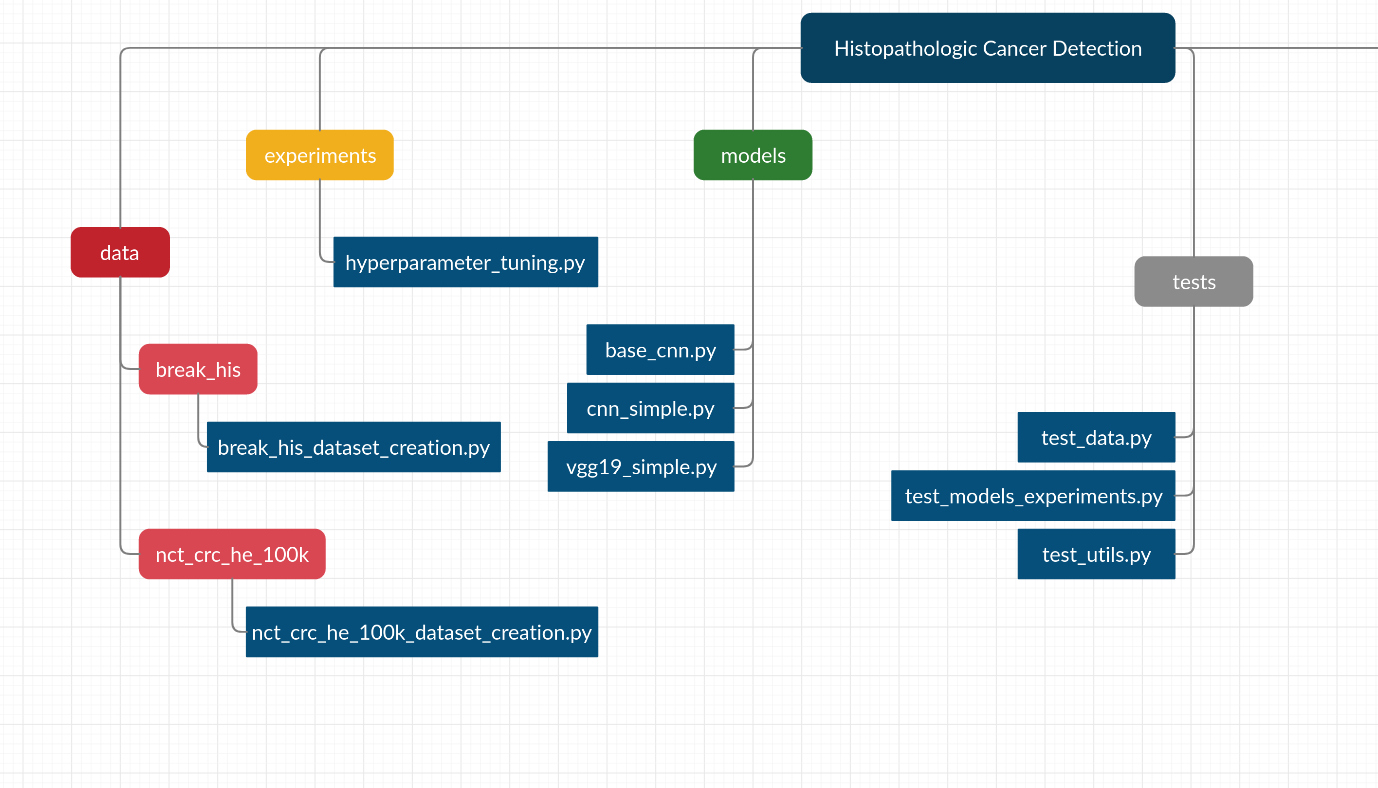
\includegraphics[scale=1.3]{code_structure_1.jpg}
	\caption{Diagram of directories and scripts of Data, Models, Experiments and Tests modules of Histopathologic Cancer Detection}
	\label{fig:dirdiag}
\end{figure}

\clearpage

\begin{figure}[h]
	\centering
	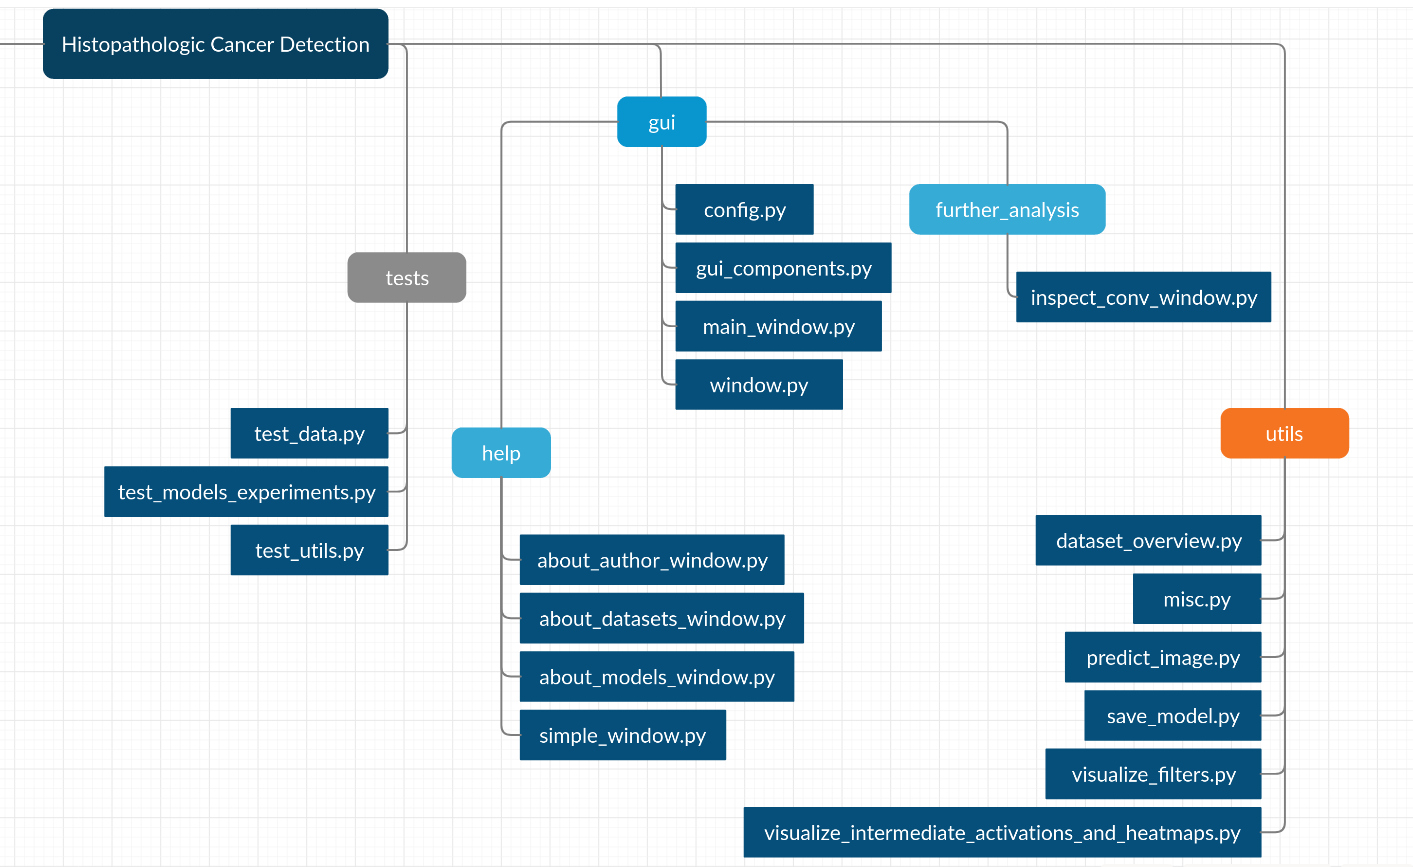
\includegraphics[scale=1.3]{code_structure_2.jpg}
	\caption{Diagram of directories and scripts of Tests, Graphical User Interface and Utilities modules of Histopathologic Cancer Detection}
	\label{fig:dirdiag2}
\end{figure}

\section{Use-Case Diagram}

One of the main goals of the Histopahtologic Cancer Detection program was the ease of use, i.e. straightforward graphical user interface which makes complex operations look quite simple and effortless. Even though there are extremely advanced algorithms with millions of parameters behind the program, GUI was made in such a way that everyone can use it. 
First step is loading the image and selecting tissue type (breast or colorectal tissue), after which classification is being done. At every step of the way, current work can be saved, and new image can be loaded to start the process from scratch. After the classification, it is possible to visualize network representations and perform further analysis of the results by visualizing layer activations, network filters and heatmap (\textcolor{red}{\autoref{fig:usecase}}).

\begin{figure}[h]
	\centering
	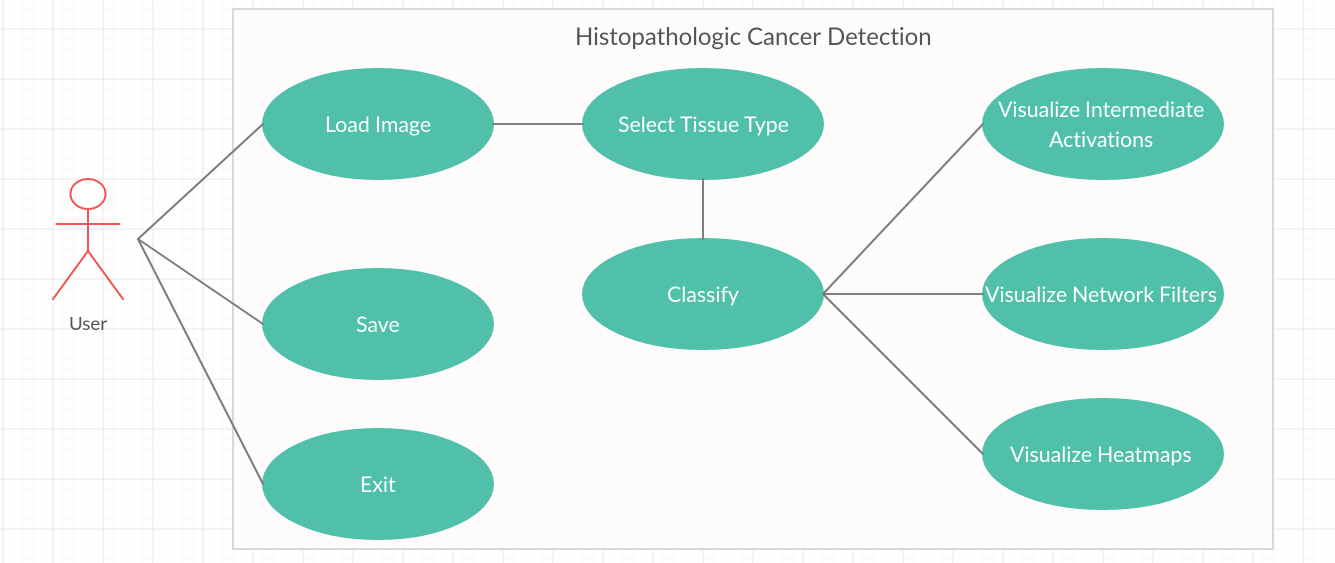
\includegraphics[scale=1.35]{use_case.jpg}
	\caption{Use-Case Diagram of Histopathologic Cancer Detection}
	\label{fig:usecase}
\end{figure}

\section{Class Diagrams}

Classes of Histopathologic Cancer Detection can be divided into two main segments: window classes and neural network classes.

BaseCNN class is the common class of all neural network classes, and it contains common attributes, such as dataset name, network name, compile parameters, and common methods, such as creation of data generators, compilation and training of the network. Neural network classes will be discussed in more detail in \textcolor{red}{\hyperref[cnn]{Section 3.5}, \hyperref[vgg19]{Section 3.6}}.

\begin{figure}[h]
	\centering
	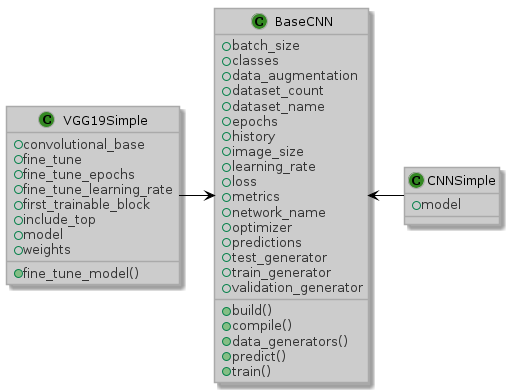
\includegraphics[scale=0.6]{nets_class_diagram.png}
	\caption{Class diagram of neural network classes of Histopathologic Cancer Detection}
	\label{fig:class1}
\end{figure}

\begin{figure}
	\centering
	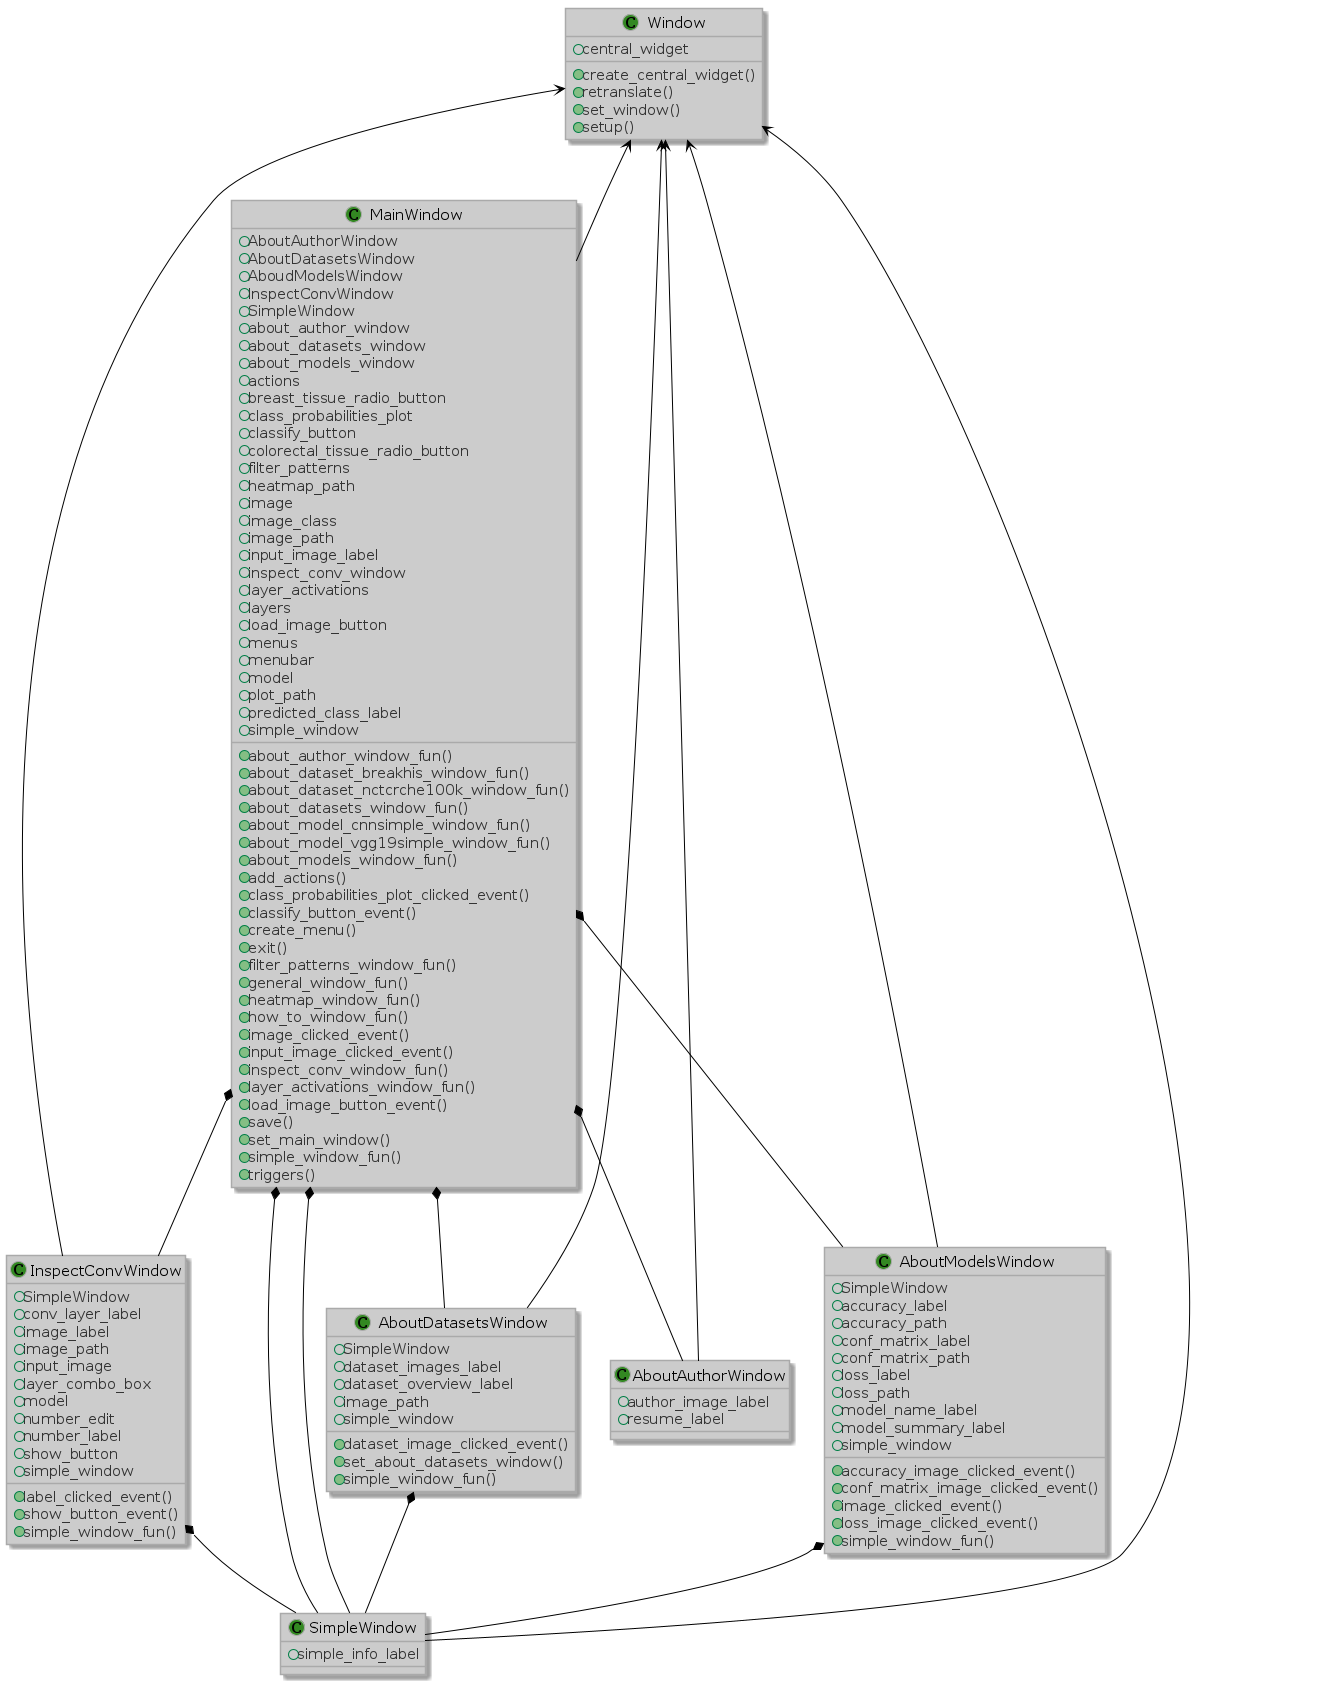
\includegraphics[scale=0.38]{main_class_diagram.png}
	\caption{Class diagram of window classes of Histopathologic Cancer Detection}
	\label{fig:class2}
\end{figure}

Window class is the base class of all window classes, and it implements common methods, such as setting up window size and central widget. On the other side, MainWindow class is the central point of GUI, as it defines the window which appears when program is run, and every other window is invoked from it (\textcolor{red}{\autoref{fig:class2}}). Window classes, along with their attributed and methods, will be discussed in more detail in \textcolor{red}{\hyperref[gui]{Section 3.8}}.

\section{Creation of Datasets}
\label{createdata}

Performance and accuracy of convolutional neural networks relies largely on datasets, i.e. on quality of available data, dataset size, class balance, etc. But before feeding data to the network, if using Keras API, certain dataset structure must be satisfied. More precisely, datasets must have the following structure: train, validation and test directories, each with subdirectory for each class. Scripts responsible for creation of required directory structure are:
\begin{itemize}
	\itemsep 0em
	\item \texttt{break\_his\_dataset\_creation.py},
	\item \texttt{nct\_crc\_he\_100k\_dataset\_creation.py}.
\end{itemize} 
They work by extracting datasets downloaded from \cite{breakhis_bib}, \cite{nctcrche100k_bib}, creating necessary directory tree and distributing images between created subdirectories. After executing scripts, datasets are ready to be fed into convolutional neural networks (in order to train them), but before that, neural network architecture has to be built.
\clearpage

\section{CNNSimple Implementation}
\label{cnn}

CNNSimple convolutional neural network (\textcolor{red}{\hyperref[src:py1]{Code 3.1}}) was created using Keras Sequential model in order to classify images from NCT-CRC-HE-100K dataset, which contains 100.000 images divided into 9 tissue/cancer categories. 

Convolutional base of CNNSimple is composed of four blocks of convolutional and max-pooling layers, where first two blocks have two convolutional and one max-pooling layer, and last two blocks have three convolutional and one max-pooling layer. Each convolutional layer has 3$\times$3 convolution window, uses ReLU activation function, and number of feature maps (filters) increases exponentially from 32 to 256. Each max-pooling layer has pool size of 2$\times$2. 

Classification top of CNNSimple is composed of two fully-connected layers, each followed by a dropout layer, and an output (also fully-connected) layer. Fully-connected layers use ReLU activation function, and number of neurons grows from 512 to 1024. Dropout layers use 50\% dropout rate (fraction of neurons which will be ignored in each passing). Output layer uses softmax activation function, and has nine neurons (one neuron per tissue/cancer subtype output). 
\vspace{1mm}
\lstset{caption={CNNSimple network architecture},label=src:py1}
\begin{lstlisting}[language={Python}, basicstyle=\scriptsize]
	model = Sequential()
	model.add(Conv2D(32, (3, 3), activation='relu', input_shape=input_shape,     
	                 name='block1_conv1'))
	model.add(Conv2D(32, (3, 3), activation='relu', name='block1_conv2'))
	model.add(MaxPooling2D((2, 2), name='block1_pool'))
	model.add(Conv2D(64, (3, 3), activation='relu', name='block2_conv1'))
	model.add(Conv2D(64, (3, 3), activation='relu', name='block2_conv2'))
	model.add(MaxPooling2D((2, 2), name='block2_pool'))
	model.add(Conv2D(128, (3, 3), activation='relu', name='block3_conv1'))
	model.add(Conv2D(128, (3, 3), activation='relu', name='block3_conv2'))
	model.add(Conv2D(128, (3, 3), activation='relu', name='block3_conv3'))
	model.add(MaxPooling2D((2, 2), name='block3_pool'))
	model.add(Conv2D(256, (3, 3), activation='relu', name='block4_conv1'))
	model.add(Conv2D(256, (3, 3), activation='relu', name='block4_conv2'))
	model.add(Conv2D(256, (3, 3), activation='relu', name='block4_conv3'))
	model.add(MaxPooling2D((2, 2), name='block4_pool'))
	model.add(Flatten(name='flatten'))
	model.add(Dense(512, activation='relu', name='dense1'))
	model.add(Dropout(0.5, name='dropout1'))
	model.add(Dense(1024, activation='relu', name='dense2'))
	model.add(Dropout(0.5, name='dropout2'))
	model.add(Dense(9, activation='softmax', name='prediction'))
\end{lstlisting} 

\section{Transfer Learning}
\label{vgg19}

Although CNNs are a powerful tool for image classification, in order to achieve high accuracy, large amount of data is needed. Problem occurs when only small dataset is available (as is often in healthcare, ex. BreakHis dataset). In such cases transfer learning can be used: take model trained on large dataset and transfer knowledge to small dataset, i.e. freeze convolutional base, and only train classification top of the network. Main idea is that early layers of convolutional base learn low-level features applicable across all images, such as edges and patterns.

\subsection{VGG19Simple Implementation}

VGG19Simple convolutional neural network (\textcolor{red}{\hyperref[src:py2]{Code 3.2}}) was created using Keras Graphical API in order to classify images from BreakHis dataset, which contains 2.081 images divided into 8 tissue/cancer categories. 

Convolutional base of VGG19Simple is VGG19 pre-built network pre-trained on ImageNet dataset (without top classification part), using imagenet weights.

Classification top of CNNSimple is composed of two fully-connected layers, each followed by a dropout layer, and an output (also fully-connected) layer. Fully-connected layers use ReLU activation function, and number of neurons grows from 512 to 1024. Dropout layers use 50\% dropout rate (fraction of neurons which will be ignored in each passing). Output layer uses softmax activation function, and has eight neurons (one neuron per tissue/cancer subtype output). 

\vspace{3mm}
\lstset{caption={VGG19Simple network architecture},label=src:py2}
\begin{lstlisting}[language={Python}, basicstyle=\scriptsize]
	input = Input((150, 150, 3))
	convolutional_base = VGG19(weights='imagenet', include_top=False,
	                           input_tensor=input)
	for layer in convolutional_base.layers:
		layer.trainable = False
	x = Flatten(name='flatten')(convolutional_base.output)
	x = Dense(512, activation='relu', name='dense_1')(x)
	x = Dropout(0.5, name='dropout_1')(x)
	x = Dense(1024, activation='relu', name='dense_2')(x)
	x = Dropout(0.5, name='dropout_2')(x)
	x = Dense(8, activation='softmax', name='predictions')(x)
	
	model = Model(input, x)
\end{lstlisting} 

\section{Experiments and Results}
\label{exp}

Performance of neural networks is determined by how well will it generalize, i.e. how high accuracy will it achieve on previously unseen data (if it performs well on training data, but underachieves on test data, it is said that CNN overfits). In order to prevent overfitting, number of techniques can be used: increase size of dataset, change network architecture or apply hyperparameter tuning techniques, which consist of selecting a set optimal hyperparameters for learning algorithm. Selection of such parameters for networks is done in \texttt{hyperparameter\_tuning.py}. First step consists of defining hyperparameter dictionary with parameters and values to be tested, such as number of epochs for which network is to be trained, optimization techniques, etc. Next step consists of training network with all combination of parameters and values defined, after which network performances are compared in order to determine the optimal hyperparameter set.

CNNSimple network trained on NCT-CRC-HE-100K dataset was trained for 50 epochs, using RMSProp optimizer with learning rate of 0.00002, using categorical crossentropy loss function. Before feeding data to the network, data augmentation (applying random transformations in order to produce more images, such as translation, rotation, sheer) has been used. In order to assess performance of the network, accuracy metrics function was employed. CNNSimple achieved 91.3\% validation and 91.3\% test accuracy, and 0.18 validation and 0.28 test loss (\textcolor{red}{\autoref{fig:cnnperf}}).

\begin{figure}[h]
	\centering
	\subfigure[\scriptsize Accuracy]{\label{fig:a}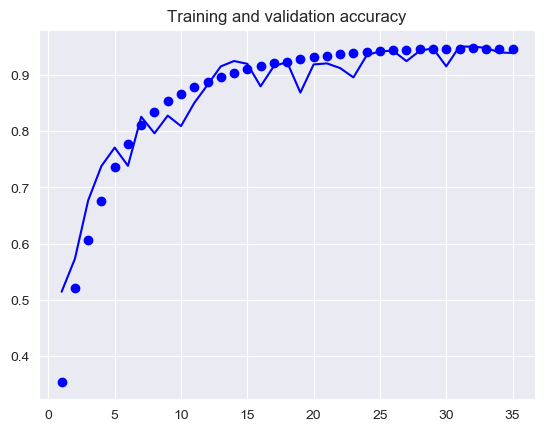
\includegraphics[width=65mm]{cnn_acc.png}}
	\subfigure[\scriptsize Loss]{\label{fig:b}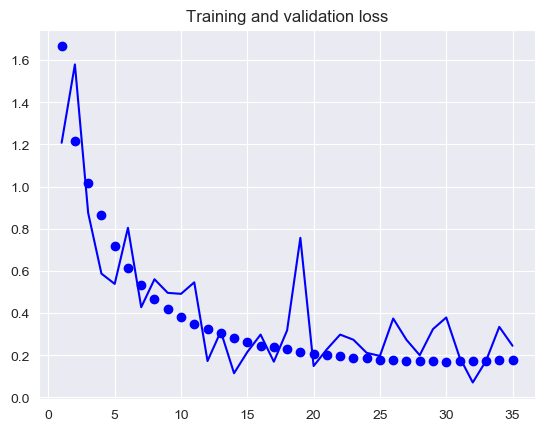
\includegraphics[width=65mm]{cnn_loss.png}}
	\caption{CNNSimple performance on NCT-CRC-HE-100K train and validation dataset}
	\label{fig:cnnperf}
\end{figure}
\clearpage

VGG19Simple network trained on BreakHis dataset was trained for 150 epochs, using Adam optimizer with learning rate of 0.0001, using categorical crossentropy loss function. Before feeding data to the network, data augmentation (applying random transformations in order to produce more images, such as translation, rotation, sheer) has been used. In order to assess performance of the network, accuracy metrics function was employed. After training network with frozen convolutional base, last convolutional block was unfreezed, and network was trained again using Adam optimizer with learning rate of 0.00005. VGG19Simple achieved 61.7\% validation and 62.1\% test accuracy, and 1.18 validation and 0.62 test loss (\textcolor{red}{\autoref{fig:vgg19perf}}).

\begin{figure}[h]
	\centering
	\subfigure[\scriptsize Accuracy]{\label{fig:vgg19perf}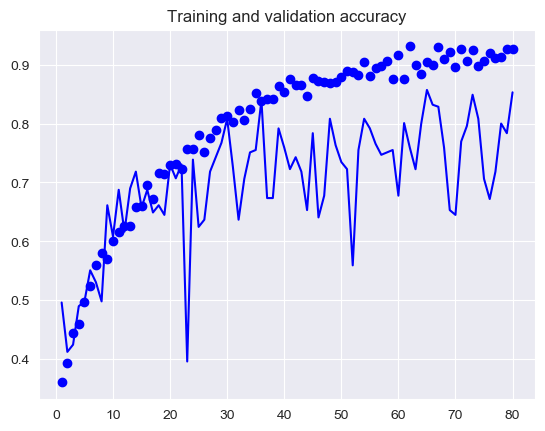
\includegraphics[width=65mm]{vgg19_acc.png}}
	\subfigure[\scriptsize Loss]{\label{fig:b}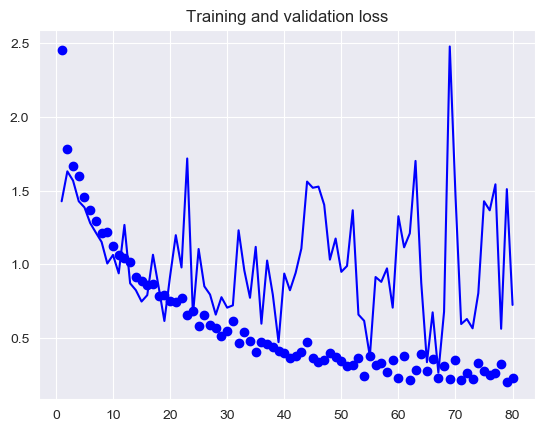
\includegraphics[width=65mm]{vgg19_loss.png}}
	\caption{VGG19Simple performance on BreakHis train and validation dataset}
	\label{fig:vgg19perf}
\end{figure}

Another way of interpreting network performance is by plotting confusion matrix, which is a summary table of correct and incorrect predictions broken down by each class (\textcolor{red}{\autoref{fig:cnncf}, \autoref{fig:vgg19cf}}).

\begin{figure}[h]
	\centering
	\begin{minipage}{.5\textwidth}
		\centering
		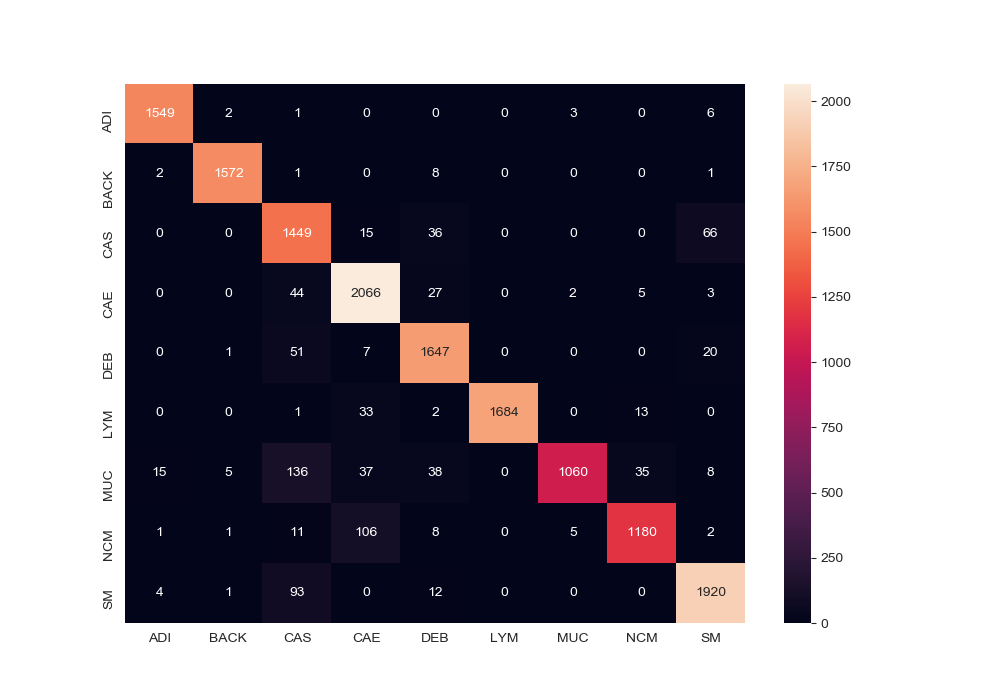
\includegraphics[scale=0.31]{cnn_cf.png}
		\captionof{figure}{Confusion Matrix of CNNSimple on NCT-CRC-HE-1OOK test dataset}
		\label{fig:cnncf}
	\end{minipage}%
	\begin{minipage}{.5\textwidth}
		\centering
		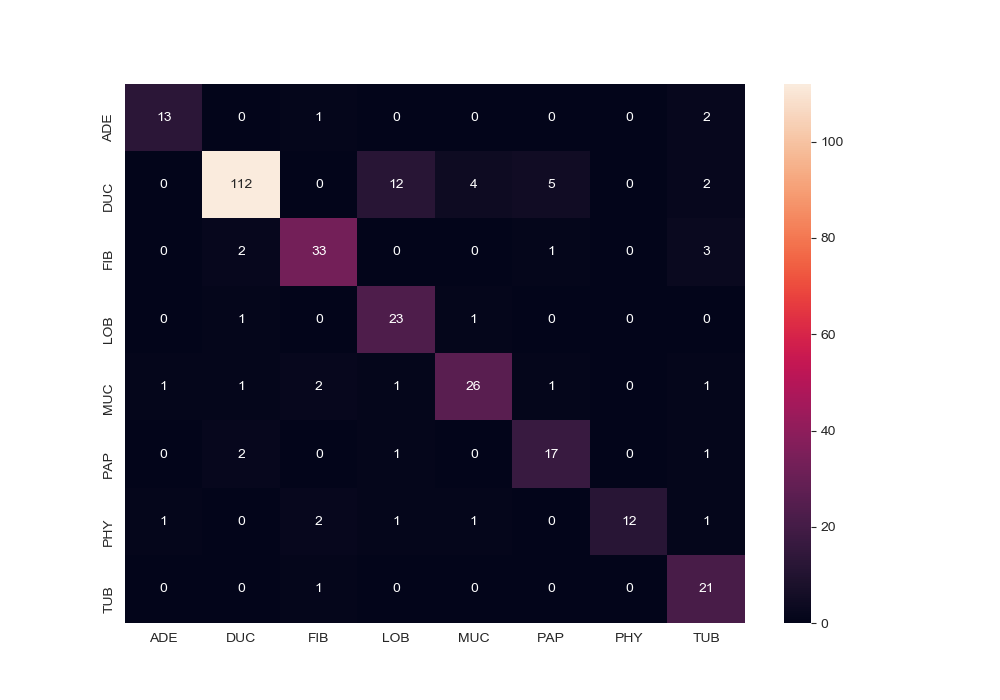
\includegraphics[scale=0.31]{vgg19_cf.png}
		\captionof{figure}{Confusion Matrix of VGG19Simple on BreakHis test dataset}
		\label{fig:vgg19cf}
	\end{minipage}
\end{figure}

\section{Graphical User Interface} 
\label{gui}

In order to make using program simple and straightforward, graphical user interface using PyQt5 has been created. Following window classes have been constructed:
\begin{itemize}
	\itemsep 0em
	\item Window class in \texttt{window.py}, used as base class for every other window, which contains primitive functions for setting up window, creating central widget, retranslating text, etc.
	\item AboutAuthorWindow class in \texttt{about\_author\_window.py}, which contains two labels (containing image and CV respectively)
	\item AboutDatasetsWindow class in \texttt{about\_datasets\_window.py}, which contains two labels (containing dataset sample images and dataset overview numbers respectively)
	\item AboutModelsWindow class in \texttt{about\_models\_window.py}, which contains five labels (containing network name, network architecture, accuracy, loss and confusion matrix plots respectively)
	\item SimpleWindow class in \texttt{simple\_window.py}, which contains one image label
	\item InspectConvWindow class in \texttt{inspect\_conv\_window.py}, which contains three labels (containing convolutional layer text, number text and image respectively), button (with associated action), combo box (containing network layer names)  and line edit (for input of numbers)
	\item MainWindow class in \texttt{main\_window.py}, which connects every other window and provides high-level program functionality 
\end{itemize}
In addition, every window-specific information is located in \texttt{config.py}, such as window sizes, positions and names of labels, paths to images, etc. GUI component definitions are located in \texttt{gui\_components.py}.

\subsection{Main Window}

MainWindow class is the central part of the GUI, as it defines the window which appears when program is started. It has menu bar from which every other window can be reached, and central widget which contains input image, tissue-type radio buttons, classify button and output class label and probabilities plot. Function \emph{classifyButtonEvent}, associated with \emph{classifyButton} is the integral part of the class, as it loads network based on the input image tissue type, classifies it, and writes output to labels.


\section{Utilities}
\label{utils}

For program to work seamlessly, certain utilities needed to be implemented:
\begin{itemize}
	\itemsep 0em
	\item \texttt{dataset\_overview.py}, used for obtaining basic information about dataset, such as sample images and image distribution per class
	\item \texttt{misc.py}, containing functions for reading file contents, loading images, etc. 
	\item \texttt{predict\_image.py}, used for predicting class to which an image belongs
	\item \texttt{save\_model.py}, used for saving neural network information and performance after being trained, such as arguments, architecture, accuracy, loss and confusion matrix plots, filters, etc.  
	\item \texttt{visualize\_filters.py}, used for visualizing network filter patterns
	\item \texttt{visualize\_intermediate\_activations\_and\_heatmaps.py}, used for visualizing intermediate activations of network and heatmaps of class activation
\end{itemize}

\section{Implementing Additional Features}

In addition to the ease of use of Histopathologic Cancer Detection program, source code was written in such a way to make expanding scope (problem space) of the program by including additional features quite simple and fast. If new tissue type (ex. lung tissue), along with tissue/cancer subtype classification was to be added to the program, it would be accomplished in four steps:
\begin{enumerate}
	\itemsep 0em
	\item \textbf{Creating dataset} \\
	Obtaining dataset of new tissue type, and preparing dataset to be fed to Keras-built CNN, which includes creating appropriate directory structure
	\item \textbf{Building CNN} \\
	Crating new convolutional neural network class inherited from BaseCNN by defining data generator transformations, network architecture, etc.
	\item \textbf{Fine-tuning CNN} \\
	Defining hyperparameter dictionary and training neural networks in order to increase classification accuracy and prevent overfitting
	\item \textbf{Extending GUI} \\
	Adding additional radio button to MainWindow class, and extending action associated with classify button, as well as further analysis actions, to use newly created network
\end{enumerate}

\section{Testing}
\label{tests}

Source code for Histopatologic Cancer Detection can be divided into two equal chunks: code responsible for CNN-related functionality and code responsible for GUI-related functionality.

Code for CNN-related functionality has been unit-tested using \texttt{PyTest} testing framework, and has a code coverage of 97\%. Unit tests for data module can be found in \texttt{test\_data.py}, unit tests for models and experiments modules can be found in \texttt{test\_models\_experiments.py}, and unit tests for utils can be found in \texttt{test\_utils.py}.

Code for GUI-related functionality has been tested manually, where numerous histopathologic slides have been loaded and classified, as well as further analyzed, in order to inspect program functionality. 

\section{External Code}

Main ideas for advanced use of Histopathologic Cancer Detection, i.e. for further analysis of CNN representations and visualization of heatmap of class activations, intermediate activations and filters of convolutional layers, as well as some parts of source code, have been taken from \cite{chollet2018deep}. Code is licensed under MIT license.